% 
% This message contains the LaTeX template for scribe notes
% in EE597.  You are free to use other means of producing
% your notes, but you are encouraged to use LaTeX: you will
% need to learn it some day.
% 
% Many thanks to Alistair Sinclair@cs.berkeley.edu for providing the basis for
% the first version of this template.
% 
% %************************************************************
%
% This is the LaTeX template file for lecture notes for EE596
% Pattern Recognition II: Introduction to Graphical Models.  When preparing 
% LaTeX notes for this class you must use this template.
%
% To familiarize yourself with this template, the body contains
% some examples of its use.  Look them over.  Then you can
% run LaTeX on this file.  After you have LaTeXed this file then
% you can look over the result either by printing it out with
% dvips or using xdvi.
%

\documentclass{article}
\usepackage{times,amsmath,amsthm,amsfonts,eucal,graphicx}

% This scribe template not only uses latex, but also
% the American Mathematical Society (AMS) latex macros.
% Detailed documentation on how to use them to produce good
% math formating can be obtained here: http://www.ams.org/tex/
% I've also placed a copy of the AMS-Latex documentation
% on the web page at:
%     http://www.ee.washington.edu/class/596/patrec/scribes/amsguide_2p.ps
% Latex documentation can be obtained from 
%
% Publications related to latex are listed here:
%     http://www.ams.org/tex/publications.html
%

\setlength{\oddsidemargin}{0.25 in}
\setlength{\evensidemargin}{-0.25 in}
\setlength{\topmargin}{-0.6 in}
\setlength{\textwidth}{6.5 in}
\setlength{\textheight}{8.5 in}
\setlength{\headsep}{0.75 in}
\setlength{\parindent}{0 in}
\setlength{\parskip}{0.1 in}

%
% The following commands set up the lecnum (lecture number)
% counter and make various numbering schemes work relative
% to the lecture number.
%
\newcounter{lecnum}
\renewcommand{\thepage}{\thelecnum-\arabic{page}}
\renewcommand{\thesection}{\thelecnum.\arabic{section}}
\renewcommand{\theequation}{\thelecnum.\arabic{equation}}
\renewcommand{\thefigure}{\thelecnum.\arabic{figure}}
\renewcommand{\thetable}{\thelecnum.\arabic{table}}

%
% A few symbols that we will be using often in this course.
\newcommand{\indep}{{\bot\negthickspace\negthickspace\bot}}
\newcommand{\notindep}{{\not\negthickspace\negthinspace{\bot\negthickspace\negthickspace\bot}}}
\newcommand{\definedtobe}{\stackrel{\Delta}{=}}
\renewcommand{\choose}[2]{{{#1}\atopwithdelims(){#2}}}
\newcommand{\argmax}[1]{{\hbox{$\underset{#1}{\mbox{argmax}}\;$}}}
\newcommand{\argmin}[1]{{\hbox{$\underset{#1}{\mbox{argmin}}\;$}}}

%
% The following macro is used to generate the header.
%
\newcommand{\lecture}[4]{
   \pagestyle{myheadings}
   \thispagestyle{plain}
   \newpage
   \setcounter{lecnum}{#1}
   \setcounter{page}{1}
   \noindent
   \begin{center}
   \framebox{
      \vbox{\vspace{2mm}
    \hbox to 6.58in { {\bf CSC 565: Graph Theory
                        \hfill North Carolina State University} }
    \hbox to 6.58in { {\bf Fall 2019
                        \hfill Dept. of Computer Science} }
       \vspace{4mm}
       \hbox to 6.28in { {\Large \hfill Lecture #1: #2  \hfill} }
       \vspace{2mm}
       \hbox to 6.28in { {\it Lecturer: {\it Prof: Don Sheehy {\tt <drsheehy@ncsu.edu>}} \hfill Scribe: #3} }
      \vspace{2mm}}
   }
   \end{center}
   \markboth{Lecture #11: #2}{Lecture #11: #2}
   \vspace*{4mm}
}

%
% Convention for citations is authors' initials followed by the year.
% For example, to cite a paper by Leighton and Maggs you would type
% \cite{LM89}, and to cite a paper by Strassen you would type \cite{S69}.
% (To avoid bibliography problems, for now we redefine the \cite command.)
% Also commands that create a suitable format for the reference list.
\renewcommand{\cite}[1]{[#1]}
\def\beginrefs{\begin{list}%
        {[\arabic{equation}]}{\usecounter{equation}
         \setlength{\leftmargin}{2.0truecm}\setlength{\labelsep}{0.4truecm}%
         \setlength{\labelwidth}{1.6truecm}}}
\def\endrefs{\end{list}}
\def\bibentry#1{\item[\hbox{[#1]}]}

%Use this command for a figure; it puts a figure in wherever you want it.
%usage: \fig{NUMBER}{CAPTION}{.eps FILE TO INCLUDE}{WIDTH-IN-INCHES}
\newcommand{\fig}[4]{
			\begin{center}
	                \includegraphics[width=#4,clip=true]{#3} \\
			Figure \thelecnum.#1:~#2
			\end{center}
	}
% Use these for theorems, lemmas, proofs, etc.
\newtheorem{theorem}{Theorem}[lecnum]
\newtheorem{lemma}[theorem]{Lemma}
\newtheorem{proposition}[theorem]{Proposition}
\newtheorem{claim}[theorem]{Claim}
\newtheorem{corollary}[theorem]{Corollary}
\newtheorem{definition}[theorem]{Definition}
% \newenvironment{proof}{{\bf Proof:}}{\hfill\rule{2mm}{2mm}}

% **** IF YOU WANT TO DEFINE ADDITIONAL MACROS FOR YOURSELF, PUT THEM HERE:

\begin{document}
%FILL IN THE RIGHT INFO.
%\lecture{**LECTURE-NUMBER**}{**DATE**}{**LECTURER**}{**SCRIBE**}
\lecture{11}{Sept 30, 2019}{Raj Shrivastava, Tanay Agrawal, Sreemoyee}
%\footnotetext{These notes are partially based on those of Nigel Mansell.}

% **** YOUR NOTES GO HERE:

% Some general latex examples and examples making use of the
% macros follow.  
%**** IN GENERAL, BE BRIEF AND COMPLETE. 
%This lecture's notes illustrate some uses of
%various \LaTeX\ macros.  
%Take a look at this and imitate.

\section{Subdivision} % Don't be this informal in your notes!
\subsection{Introduction}

The two graphs G and H shown in fig~\ref{fig:fig1} are not isomorphic. This is because the number of edges and the number of vertices are not same, which is an invariant for finding isomorphism among graphs.

\begin{figure}[h]
    \centering
    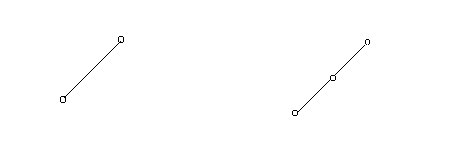
\includegraphics[width=0.5\textwidth]{images/fig1.png}
    \caption{Two graphs G and H}
    \label{fig:fig1}
\end{figure}

From figure \ref{fig:fig1}, the relation between graphs these graphs can be extended to geometric realisation as:

\begin{table}[h]
\begin{center}
\begin{tabular}{lll}
G       & $\cong$ & H      \\
$\downarrow$ &  &  $\downarrow$  \\
geom(G) & $\cong$ & geom(H)
\end{tabular}

\end{center}
\end{table}


On the other hand, if we take the geometric realization of these two graphs, we find that those are homeomorphic i.e. there exists a continuous mapping from all the vertices in geometric realization of G to all the vertices in geometric realization of H in the topological space.

\begin{figure}[h]
    \centering
    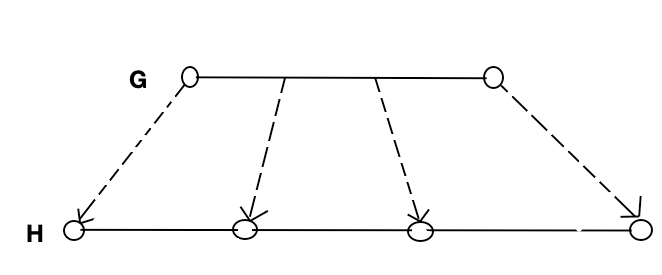
\includegraphics[width=0.5\textwidth]{images/fig3.png}
    \caption{Homeomorphism b/w geom(G) and geom(H)}
    \label{fig:}
\end{figure}

\subsection{Understanding Subdivision}

H is a subdivision of G if it is formed from G by subdividing zero or more number of edges.

If we can take one edge of a graph and keep on subdividing it, the resultant graph will be a subdivision of the initial graph. Geometric realizations for the initial graph and the final graph (after subdivision) will be homeomorphic to each other.

If we recall, the Eulerian characteristic for graphs is:

$e(G) = |V_G| - |E_G|$

There is an interesting fact for subdivision with regard to Eulerian Characteristic.

\textbf{Fact}: If G is a subdivision of H, then $$e(G) = e(H)$$

The reason behind such characteristic is that if we subdivide an edge once, the number of edges and the number of vertices both increase by one. Similarly, if we contract an edge once, the number of edge and the number of vertices both decrease by one.

\section{Topological Minor}
\subsection{\textbf{Definition}}
G is a topological minor of H, if H contains a sub graph which is a subdivision of G.

\textbf{Example 1} : Consider the following two graphs G and H.
\begin{figure}[!h]
    \centering
    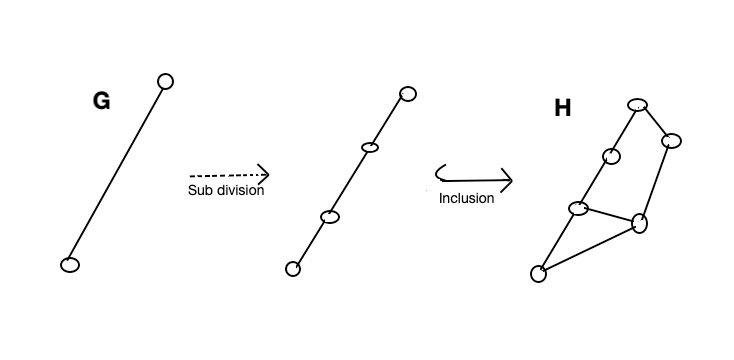
\includegraphics[width=0.76\textwidth]{images/topMinorDef.png}
    \caption{Graph G is a topological minor of Graph H}
    \label{fig:topMinorDef}
\end{figure}


In figure ~\ref{fig:topMinorDef}, an intermediate graph is formed by subdividing the graph G and then including that into a larger graph H through inclusion (the intermediate graph becomes a subgraph of H). Thus, we can say that graph G is a topological minor of graph H.

\textbf{Example 2} : Consider the following two graphs G ($K_4$) and H. 

\begin{figure}[h]
    \centering
    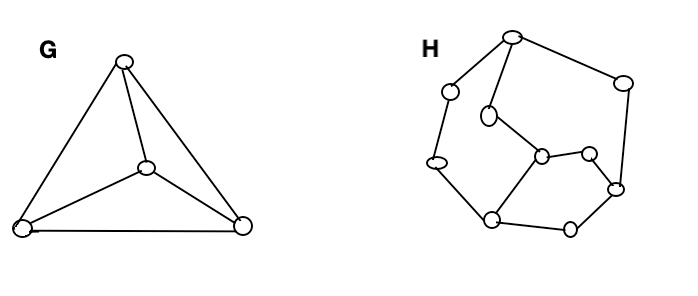
\includegraphics[width=0.5\textwidth]{images/G_sub_K4.png}
    \caption{G is a sub division of H.}
    \label{fig:G_sub_K4}
\end{figure}

In figure ~\ref{fig:G_sub_K4}, H is formed by subdividing G, i.e., the edges of G are sub divided to form H.

\textbf{Example 3}: Consider the following two graphs G ($K_4$) and H.

\begin{figure}[!h]
    \centering
    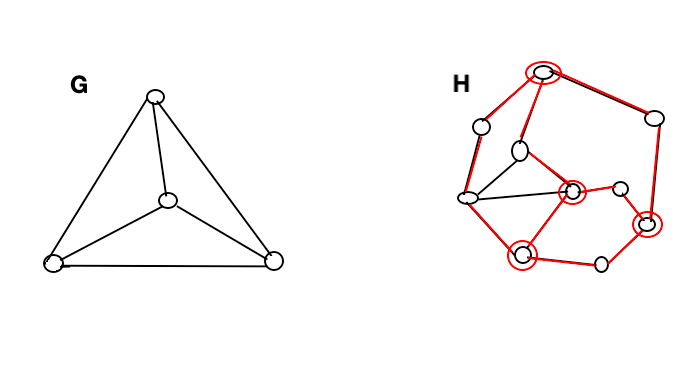
\includegraphics[width=0.5\textwidth]{images/G_notSub_K4.png}
    \caption{Graph G ($K_4$) is a topological minor of Graph H}
    \label{fig:G_notSub_K4}
\end{figure}

In figure ~\ref{fig:G_notSub_K4}, H is not a subdivision of G, but G is still a topological minor of H. 

The graph highlighted with red edges and red vertices is actually a subgraph of H and was formed by subdividing graph G. Thus, by definition, we can say that graph G is a topological minor of graph H.

Subdivision and inclusion follow \textbf{partial ordering} in case of topological minor.

For a relation to be a Partial order, it has to be:
\begin{itemize}
    \item Anti-Symmetric
    \item Reflexive
    \item Transitive
\end{itemize}

\subsection{\textbf{Transitivity in topological minors}}
Topological transitivity is denoted by $\preceq _T$ is transitive.\\
Transitivity here means that if A $\preceq _T$ B and B $\preceq_T$ C, then A $\preceq _T$ C.

\begin{figure}[!h]
    \centering
    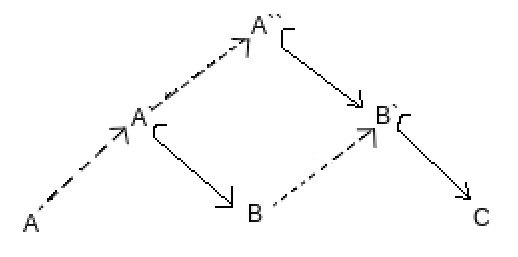
\includegraphics[width=0.4\textwidth]{images/top_transitivity.png}
    \caption{Transitivity in topological minor}
    \label{fig:}
\end{figure}


\section{Contraction}
\subsection{Introduction}
\begin{figure}[!h]
    \centering
    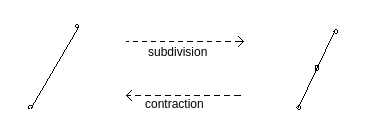
\includegraphics[width=0.5\textwidth]{images/contraction-1.png}
    \caption{Special case of contraction}
    \label{fig:contraction-1}
\end{figure}

Figure ~\ref{fig:contraction-1} shows a special case of contraction, as this contraction can actually be considered as reverse of subdivision which is not true always.

\begin{figure}[!h]
    \centering
    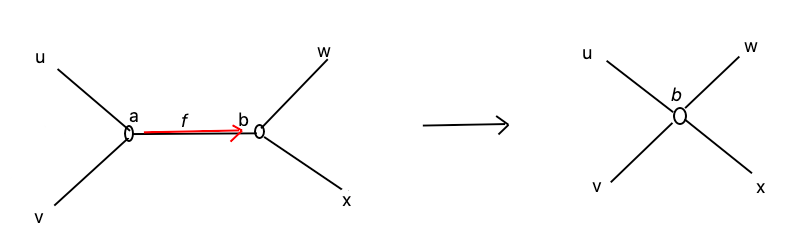
\includegraphics[width=0.5\textwidth]{images/contraction-2.png}
    \caption{Contraction}
    \label{fig:contraction-2}
\end{figure}

Contraction can be understood more like a function rather than an operation. From figure-\ref{fig:contraction-2}, the function $f$ can be defined as:

$f_v(a) = b$ and $f_s(\sigma) = \{f_v(u): u \in \sigma \}$

\begin{figure}[!h]
    \centering
    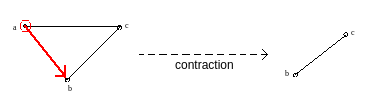
\includegraphics[width=0.5\textwidth]{images/contraction-3.png}
    \caption{General case of contraction}
    \label{fig:gen_cont}
\end{figure}

\subsection{\textbf{Definition}}
A contraction is a surjective simplicial map such that pre-images of connected sub graphs are connected. Also, G is a contraction of H if there is a contraction H$\rightarrow$ G.

From this definition, it follows that the contraction of a contraction is also a contraction.
\begin{figure}[!h]
    \centering
    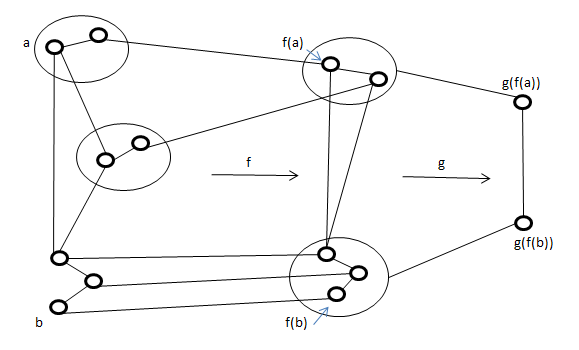
\includegraphics[width=0.5\textwidth]{images/Compose_Contraction.png}
    \caption{Graph H is a sub division of Graph G}
    \label{fig:Compose_Contraction}
\end{figure}

In figure ~\ref{fig:Compose_Contraction}, we have two contraction maps , f and g. We want to find a path from a to b using the fact that they are connected in the contraction g of f.

Next, we compose a path from f(a) to f(b) using the fact that the set of vertices in the pre-images are connected and taking the path between
these the sets which contain f(a) and f(b) respectively. Extending this to the first graph, we can find the path between vertices a and b in similar fashion.

%\fig{6}{Transitivity in contraction}{\images\}{1.5in}{1.5in}

\subsection{\textbf{Minor}}
G is a minor of H if G is a contraction of a sub graph of H

$G \preceq H \iff$ G is a minor of H 

\begin{figure}[!h]
    \centering
    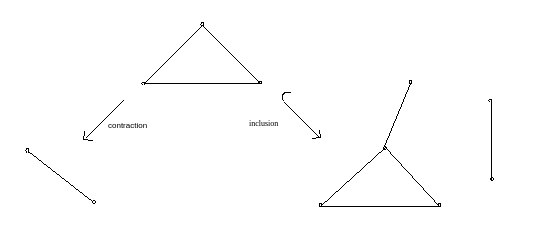
\includegraphics[width=0.78\textwidth]{images/Fig_(last-1).png}
    \caption{Minor in graphs}
    \label{fig:}
\end{figure}

\textbf{Claim}: $\preceq$ is transitive

\begin{figure}[!h]
    \centering
    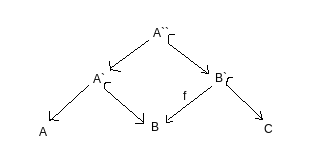
\includegraphics[width=0.5\textwidth]{images/Fig_last.png}
    \caption{Transitivity in minors}
    \label{fig:Fig_last}
\end{figure}

An interesting fact to be noted from the figure ~\ref{fig:Fig_last} is that A` is a minor of B`.

\textbf{Claim}: If G is a topological minor of H, then G is a minor of H.

However, the converse does not necessarily hold.

Topological minors are subsets of all minors of a graph.

\begin{theorem}
$geom(G) \cong geom(H)$ iff there exists some common subdivision, i.e. a graph X such that X is a subdivision of G and H.
\end{theorem}
\begin{proof}
Euler characteristic is a topological invariant.\\
If X is a subdivision of G, then
\begin{equation}
    e(X) = e(G)
\end{equation}
Similarly, if X is a subdivision of H then
\begin{equation}
    e(X) = e(H)
\end{equation}
By eqn 11. and eqn 11.2,\\
e(G) = e(H)\\
$\implies geom(G) \cong geom(H)$
\end{proof}
% **** THIS ENDS THE EXAMPLES. DON'T DELETE THE FOLLOWING LINE:

\end{document}